\chapter{Calculer des durées}
{https://sacado.xyz/qcm/parcours_show_course/0/117137}
{ 

\begin{CpsCol}
\textbf{ Les savoir-faire du parcours}
 \begin{itemize}
 \item Savoir convertir des durées.
 \item Savoir effectuer des opérations avec des durées.
 \item Savoir convertir des heures décimales.
 \item Savoir résoudre un problème de durée. 
 \end{itemize}
\end{CpsCol}

}

\begin{pageCours} 

\section{Heures, minutes, secondes}

\begin{DefT}{Système horaire}
Notre système de mesure des heures, minutes et secondes est un \textbf{système sexagésimal}\index{système sexagésimal}.
\begin{center}
 $1$ heure=$60$ minutes\hspace{1cm}$1$ minute=$60$ secondes 
\end{center}
\end{DefT}

\begin{Mt}
\textbf{Transformation de $451$ minutes en heures et minutes.}

En effectuant la division euclidienne
$\opidiv{451}{60}$

on trouve :
$451=7\times60+31$ donc $451$ minutes = $7$ heures et $31$ minutes.
\end{Mt}



\section{Millénaires, siècles, années, mois}

\begin{Def}
 Un millénaire = $1000$ ans \hspace{0.35cm} Un siècle = $100$ ans \hspace{0.35cm} Une année = $12$ mois  \hspace{0.35cm}  Une semaine = $7$ jours
\end{Def}

\begin{Def}
  Un jour = $24$ heures \hspace{0.5cm} Une heure = $60$ minutes\hspace{0.5cm} Une minute = $60$ secondes
\end{Def}

\begin{Mt}
\textbf{Transformation de 713 heures en semaines, jours et heures}.

Comme on souhaite convertir en semaine, il est nécessaire de connaitre le nombre d'heures en une semaine : 

Une semaine = 7 jours = $7\times 24$ heures = $168$ heures.

\begin{minipage}{0.4\linewidth}
$\opidiv{713}{168}$
\end{minipage}
\begin{minipage}{0.4\linewidth}
$\opidiv{41}{24}$
\end{minipage}

$713$ heures  = $4 \times 168 + 41$ donc  $713$ heures  = $4$ semaines + $41$ heures

$41$ heures = $1 \times 24$ + $17$  heures = $1$ jour  + $17$ heures

On trouve donc $713$  heures = $4$ semaines, $1$ jour, $17$ heures.
\end{Mt}



\end{pageCours}

\begin{pageAD}

\Sf{Convertir des heures, minutes, secondes}

 
\begin{ExoCad}{Communiquer}

\begin{minipage}{0.58\linewidth}
Combien font $235$ s en minutes et secondes ? 
 
\point{3}
\end{minipage}
\hfill
\vrule
\hfill
\begin{minipage}{0.38\linewidth}
Opérations
\vspace{2.5cm}
\end{minipage}

\end{ExoCad}
 

\begin{ExoCad}{Communiquer}

\begin{minipage}{0.58\linewidth}
Combien font $34 990$ s en heures, minutes et secondes ? \point{4}
 
\end{minipage}
\hfill
\vrule
\hfill
\begin{minipage}{0.38\linewidth}
Opérations
\vspace{2.5cm}
\end{minipage}

\end{ExoCad}

\Sf{Connaître et utiliser les unités de mesure des durées et leurs relations.}
 
\begin{ExoCad}{Communiquer}

\begin{minipage}{0.58\linewidth}
Transformer $1024$ secondes en heures, minutes et secondes. 
 
\point{3}
\end{minipage}
\hfill
\vrule
\hfill
\begin{minipage}{0.38\linewidth}
Opérations
\vspace{2.5cm}
\end{minipage}


\end{ExoCad}

\begin{ExoCad}{Communiquer}

\begin{minipage}{0.58\linewidth}
Transformer 868 heures en semaines, jours et heures. 
 
\point{3}
\end{minipage}
\hfill
\vrule
\hfill
\begin{minipage}{0.38\linewidth}
Opérations
\vspace{2.5cm}
\end{minipage}


\end{ExoCad}


\end{pageAD}


\begin{pageCours}
\section{Opérations avec des durées}

\subsection{Ajouter des durées}

\begin{Mt}
Pour ajouter des durées on ajoute les heures entre elles et les minutes entre elles puis on convertit l'excédent de minutes en heures et minutes :

\begin{minipage}{0.15\linewidth}
\begin{tabular}{ccccc} 
& 04 & h & 54 & min \\ 
+  & 07 & h & 41 & min\\ 
\hline 
& 11 & h & 95 & min \\
\end{tabular} 
\end{minipage}
\hfill
\begin{minipage}{0.7\linewidth}
  $11$h$95$min = $11$h + $60$ min + $35$ min 
 
  $11$h$95$min =$11$h + $1$ h + $35$ min 
 
  $11$h$95$min = $12$h + $35$ min
\end{minipage}

\end{Mt}
%\begin{Mt}
%On peut aussi transformer toutes les données en minutes puis convertir en heures et minutes une fois le calcul effectué :
%
%$04h54min+07h41min=4\times60+54+7\times60+41=755min$
%
%Puis : $755=12\times60+35$. Ainsi : $04h54min+07h41min=12h35min$
%\end{Mt}



\subsection{Soustraire des durées}

\begin{Mt}
Pour soustraire des durées, on soustrait les heures entre elles et les minutes entre elles. Si {\color{sacado_red} le nombre de minutes} soustrait est plus petit que le {\color{sacado_blue} nombre de minutes à soustraire} on convertit la première durée en lui décalant une heure en minutes.
 
\begin{minipage}{0.23\linewidth}
\begin{tabular}{ccccc} 
& $05$ & h & {\color{sacado_red}$33$} & min \\ 
$-$   & $03$ & h & {\color{sacado_blue}$55$} & min\\ 
\hline 
\end{tabular} 
\end{minipage}
\hfill
\begin{minipage}{0.07\linewidth}
\begin{center}
s'écrit :  
\end{center}
\end{minipage}
\hfill
\begin{minipage}{0.23\linewidth}
\begin{tabular}{ccccc} 
& {\color{sacado_green}$04$} & h & {\color{sacado_green}$93$} & min \\ 
$-$   & $03$ & h &  {\color{sacado_blue}$55$} & min\\ 
\hline 
& 1 & h & 38 & min \\
\end{tabular}
\end{minipage}
\hfill
\begin{minipage}{0.35\linewidth}
Donc $05$ h $33$ min $-$ $03$ h $55$ min 

= $01$ h $38$ min
\end{minipage}

\end{Mt}



\section{Heure en système décimal (Limite du programme)}

\begin{Def}
On peut exprimer des heures en utilisant le \textbf{système décimal}.
\end{Def}

\begin{Mt}
Pour convertir $2,20h$ en heures et minutes on exprime la partie décimale du nombre en minutes en utilisant la \textbf{proportionnalité} :
\begin{tabular}{|c|c|c|}\hline
Durée (h) & 1 & 0,2\\ \hline
Durée (min) & 60 & 12\\ \hline
\end{tabular}

D'après la proportionnalité, $0,20 heure = 0,20\times60=12min$. Ainsi : $2,20h=2h12min$
\end{Mt}


\end{pageCours}




\begin{pageAD}


\Sf{Déterminer un instant à partir de la connaissance d'un instant et d'une durée.} 


\begin{ExoCad}{Représenter. Calculer.}
 Effectue les sommes suivantes :
 
\begin{minipage}{0.30\linewidth}
\begin{tabular}{ccccc} 
& $03$ & h &  $34$ & min \\ 
$+$   & $05$ & h & $22$  & min\\ 
\hline 
   &  & h & & min\\
\end{tabular} 
\end{minipage}
\hfill 
\begin{minipage}{0.30\linewidth}
 \begin{tabular}{ccccc} 
& $02$ & h &  $50$ & min \\ 
$+$   & $07$ & h &  $28$ & min\\ 
\hline 
   &  & h & & min\\
\end{tabular} 
\end{minipage}
\hfill 
\begin{minipage}{0.30\linewidth}
 \begin{tabular}{ccccc} 
& $04$ & h & $47$  & min \\ 
$+$   & $15$ & h & $16$ & min\\ 
\hline 
   &  & h & & min\\
\end{tabular} 
\end{minipage}
 
\end{ExoCad}

\Sf{Calculer la durée écoulée entre deux instants donnés}


\begin{ExoCad}{Représenter. Calculer.}

 Effectue les différences suivantes :
 
 
 \begin{minipage}{0.30\linewidth}
\begin{tabular}{ccccc} 
& $05$ & h &  $43$ & min \\ 
$-$   & $01$ & h & $22$ & min\\ 
\hline 
   &  & h & & min\\
\end{tabular} 
\end{minipage}
\hfill 
\begin{minipage}{0.30\linewidth}
 \begin{tabular}{ccccc} 
& $15$ & h &  $12$ & min \\ 
$-$   & $07$ & h &  $38$ & min\\ 
\hline 
   &  & h & & min\\
\end{tabular} 
\end{minipage}
\hfill 
\begin{minipage}{0.30\linewidth}
 \begin{tabular}{ccccc} 
& $11$ & h & $27$  & min \\ 
$-$   & $5$ & h & $43$ & min\\ 
\hline 
   &  & h & & min\\
\end{tabular} 
\end{minipage}
 
\end{ExoCad}

\Sf{Résoudre des problèmes en exploitant des ressources variées  }


\begin{minipage}{0.49\linewidth}

\begin{ExoCad}{Représenter. Calculer.}

Le journal d'une chaine télévisée débute à $19$h$45$ et se termine à $20$h$21$. Quelle est la durée du JT ?
 \point{5}
 \end{ExoCad}
\end{minipage}
\hfill 
 \begin{minipage}{0.49\linewidth}
\begin{ExoCad}{Représenter. Calculer.}

Un groupe de cycliste est partie à $8$h$34$ et a roulé pendant $2$h$42$. A quelle heure le groupe est-il arrivé  ?
 \point{5}
\end{ExoCad}
\end{minipage}

 


  


\begin{ExoCad}{Chercher. Calculer.}

\begin{minipage}{0.70\linewidth}
Voici les horaires d'ouverture d'un parking. Quelle est sa durée d'ouverture le dimanche ? \point{4}
\end{minipage}
\begin{minipage}{0.30\linewidth}
 
 \begin{center}
 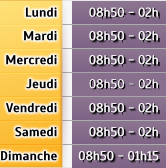
\includegraphics[scale=0.7]{FIG/grandeurs_mesures/horaires_parking.jpg} 
 \end{center}
\end{minipage}

\end{ExoCad}

\end{pageAD}

%%%%%%%%%%%%%%%%%%%%%%%%%%%%%%%%%%%%%%%%%%%%%%%%%%%%%%%%%%%%%%%%%%%%%%%%%%%%%%%%%%%%%%%%%%%%%%%%%%%%%
%%%%%%%%%% Parcours 1
%%%%%%%%%%%%%%%%%%%%%%%%%%%%%%%%%%%%%%%%%%%%%%%%%%%%%%%%%%%%%%%%%%%%%%%%%%%%%%%%%%%%%%%%%%%%%%%%%%%%%
\begin{pageParcoursu}

\ExoCu{Représenter. Calculer.}

 Complète les égalités :\vspace{0.2cm}
 \begin{itemize}
 \item $2$ siècles =  $\ldots\ldots \times \ldots \ldots $ années = $\ldots \ldots \ldots\ldots$ années \vspace{0.2cm}
 \item $4$ millénaires = $\ldots \ldots\times \ldots \ldots $ mois =$\ldots \ldots\ldots\ldots $ mois \vspace{0.2cm}
 \item $6$ années = $\ldots\ldots \times \ldots \ldots $ mois = $\ldots \ldots\ldots\ldots$ mois \vspace{0.2cm}
 \end{itemize}

\ExoCu{Représenter. Calculer.}

Convertis les durées données :\vspace{0.2cm}

\begin{minipage}{0.50\linewidth}
 \begin{itemize}
 \item $6$h$00$ =  $\ldots \ldots\ldots\ldots $ min.  \vspace{0.2cm}
 \item $2$h$15$ =  $\ldots \ldots\ldots\ldots $ min. \vspace{0.2cm}
 \item $5$h$45$=  $\ldots \ldots\ldots\ldots $ min. \vspace{0.2cm}
 \end{itemize}
\end{minipage}
\begin{minipage}{0.50\linewidth}
 \begin{itemize}
 \item $90$ minutes  =  $\ldots \ldots \ldots \ldots $ h $\ldots \ldots \ldots \ldots $ min. \vspace{0.2cm}
 \item $120$ minutes = $\ldots \ldots \ldots \ldots $ h $\ldots \ldots \ldots \ldots $ min. \vspace{0.2cm}
 \item $180$ minutes = $\ldots \ldots \ldots \ldots $ h $\ldots \ldots \ldots \ldots $ min. \vspace{0.2cm}
 \end{itemize}
\end{minipage}



\ExoCu{Calculer.}
 
 Effectue  les sommes suivantes :
 
\begin{minipage}{0.30\linewidth}
\begin{tabular}{ccccc} 
& $04$ & h &  $14$ & min \\ 
$+$   & $01$ & h & $25$  & min\\ 
\hline 
   &  & h & & min\\
\end{tabular} 
\end{minipage}
\hfill 
\begin{minipage}{0.30\linewidth}
 \begin{tabular}{ccccc} 
& $05$ & h &  $10$ & min \\ 
$+$   & $03$ & h &  $28$ & min\\ 
\hline 
   &  & h & & min\\
\end{tabular} 
\end{minipage}
\hfill 
\begin{minipage}{0.30\linewidth}
 \begin{tabular}{ccccc} 
& $05$ & h & $22$  & min \\ 
$+$   & $12$ & h & $06$ & min\\ 
\hline 
   &  & h & & min\\
\end{tabular} 
\end{minipage}
 
 
 
\ExoCu{Calculer.}

Effectue  les différences suivantes :
 
 
 \begin{minipage}{0.30\linewidth}
\begin{tabular}{ccccc} 
& $05$ & h &  $22$ & min \\ 
$-$   & $04$ & h & $12$ & min\\ 
\hline 
   &  & h & & min\\
\end{tabular} 
\end{minipage}
\hfill 
\begin{minipage}{0.30\linewidth}
 \begin{tabular}{ccccc} 
& $04$ & h &  $13$ & min \\ 
$-$   & $02$ & h &  $12$ & min\\ 
\hline 
   &  & h & & min\\
\end{tabular} 
\end{minipage}
\hfill 
\begin{minipage}{0.30\linewidth}
 \begin{tabular}{ccccc} 
& $15$ & h & $27$  & min \\ 
$-$   & $12$ & h & $13$ & min\\ 
\hline 
   &  & h & & min\\
\end{tabular} 
\end{minipage}
 

\ExoCu{Calculer.}
 
 Axel part de lui chez à $7$h$42$ pour aller au collège. Il marche pendant $9$ minutes. A quelle heure arrive-t-il à son collège ?
\point{4}


\ExoCu{Calculer.}

\begin{minipage}{0.60\linewidth} 
 Quelle est la différence entre ces deux horaires ?
\point{4}
\end{minipage}
\hfill 
\begin{minipage}{0.40\linewidth}
 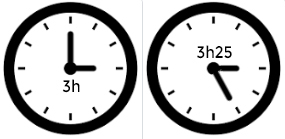
\includegraphics[scale=1]{FIG/grandeurs_mesures/heure_delta.jpg} 
\end{minipage}



\end{pageParcoursu}

%%%%%%%%%%%%%%%%%%%%%%%%%%%%%%%%%%%%%%%%%%%%%%%%%%%%%%%%%%%%%%%%%%%%%%%%%%%%%%%%%%%%%%%%%%%%%%%%%%%%%
%%%%%%%%%% Parcours 2
%%%%%%%%%%%%%%%%%%%%%%%%%%%%%%%%%%%%%%%%%%%%%%%%%%%%%%%%%%%%%%%%%%%%%%%%%%%%%%%%%%%%%%%%%%%%%%%%%%%%%
\begin{pageParcoursd}

\ExoCd{Calculer.}
 
 Effectue  les opérations suivantes :
 
\begin{minipage}{0.30\linewidth}
\begin{tabular}{ccccc} 
& $04$ & h &  $44$ & min \\ 
$+$   & $02$ & h & $25$  & min\\ 
\hline 
   &  & h & & min\\
\end{tabular} 
\end{minipage}
\hfill 
\begin{minipage}{0.30\linewidth}
 \begin{tabular}{ccccc} 
& $15$ & h &  $33$ & min \\ 
$+$   & $04$ & h &  $51$ & min\\ 
\hline 
   &  & h & & min\\
\end{tabular} 
\end{minipage}
\hfill 
\begin{minipage}{0.30\linewidth}
 \begin{tabular}{ccccc} 
& $15$ & h & $22$  & min \\ 
$-$   & $2$ & h & $45$ & min\\ 
\hline 
   &  & h & & min\\
\end{tabular} 
\end{minipage}



\ExoCd{Chercher. Calculer.}


\begin{minipage}{0.62\linewidth}
 Sur un site Internet, on trouve le trajet entre Hyères et Chambéry. Pierre décide de partir à $10$h$30$ de Hyères. A quelle va-t-il arriver à Chambéry ?
 \point{6}
\end{minipage}
\hfill 
\begin{minipage}{0.35\linewidth}
  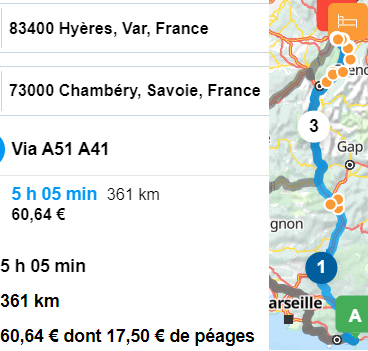
\includegraphics[scale=0.7]{FIG/grandeurs_mesures/via_michelin.jpg} 
\end{minipage}


 \ExoCd{Chercher. Calculer.} 
 
 Voici les horaires de train entre Castres et Toulouse. Complète le tableau.
 
 \begin{minipage}{0.5\linewidth}
 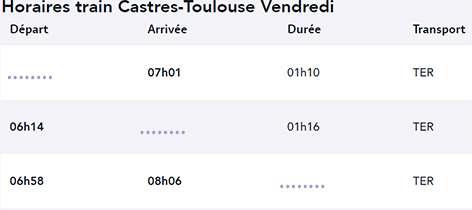
\includegraphics[scale=1]{FIG/grandeurs_mesures/castres_toulourse_train.jpg} 
 \end{minipage}
\begin{minipage}{0.5\linewidth}
  Opérations :
  \vspace{5cm}
\end{minipage}
 


\ExoCd{Représenter. Calculer.}


Depuis 2020, en TOP 14, la durée de pause à la mi-temps est de 20 minutes et le match dure deux mi-temps de $40$ minutes chacune. Un match commence à $21$h$05$.  A quelle heure finit le match de Top 14 ? \point{6}


 
\end{pageParcoursd}
%%%%%%%%%%%%%%%%%%%%%%%%%%%%%%%%%%%%%%%%%%%%%%%%%%%%%%%%%%%%%%%%%%%%%%%%%%%%%%%%%%%%%%%%%%%%%%%%%%%%%
%%%%%%%%%% Parcours 3
%%%%%%%%%%%%%%%%%%%%%%%%%%%%%%%%%%%%%%%%%%%%%%%%%%%%%%%%%%%%%%%%%%%%%%%%%%%%%%%%%%%%%%%%%%%%%%%%%%%%%
\begin{pageParcourst}

 \ExoCt{Chercher. Calculer.} 

Ne le sait-on pas mais il y a des marée en Méditerranée ? Et oui ! A Hyères, on relève le tableau de marée suivant.

 \begin{minipage}{10cm}
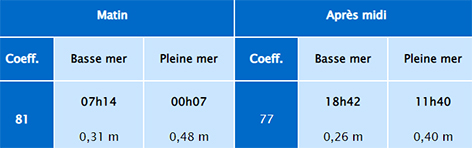
\includegraphics[scale=0.7]{FIG/grandeurs_mesures/maree.jpg} 

Quelle est la durée entre la pleine mer et la basse mer du matin ? \point{2}

Quelle est la durée entre la pleine mer et la basse mer de l'après midi ? \point{2}


 \end{minipage}
\begin{minipage}{5cm}
  Opérations :
  \vspace{6cm}
\end{minipage}



 
\ExoCt{Chercher. Calculer.} 

Gustav Iden a remporté l’Iron Man Floride avec un temps de $7$h$42$min$57$s et Kristian Blummenfelt a établi le temps Ironman le plus rapide jamais enregistré à Cozumel. Pour mettre cette performance en perspective, voici ses temps :

\begin{itemize}
\item 39: 41 en natation
\item 4: 02: 40 en vélo
\item 2:  35: 24 en course à pied
\end{itemize}

Quel est le temps total de Kristian Blummenfelt lors de son triathlon ?\point{6}


\ExoCt{Communiquer.}

\begin{enumerate}
 
\item Convertir les heures décimales suivantes en heures et minutes :
 
 \begin{itemize}
\item $3,2$h = $\ldots\ldots\ldots\ldots\ldots\ldots\ldots\ldots\ldots$
\item $4,1$h = $\ldots\ldots\ldots\ldots\ldots\ldots\ldots\ldots\ldots$
\item $7,6$h = $\ldots\ldots\ldots\ldots\ldots\ldots\ldots\ldots\ldots$
\item $3,25$h = $\ldots\ldots\ldots\ldots\ldots\ldots\ldots\ldots\ldots$
\end{itemize}
 
\item  Convertir les heures et minutes suivantes en heures décimales :
 \begin{itemize}
\item $3$h$20$min = $\ldots\ldots\ldots\ldots\ldots\ldots\ldots\ldots\ldots$
\item $1$h$55$min = $\ldots\ldots\ldots\ldots\ldots\ldots\ldots\ldots\ldots$
\item $2$h$13$min = $\ldots\ldots\ldots\ldots\ldots\ldots\ldots\ldots\ldots$
\end{itemize} 

\end{enumerate}
  
\end{pageParcourst}

%%%%%%%%%%%%%%%%%%%%%%%%%%%%%%%%%%%%%%%%%%%%%%%%%%%%%%%%%%%%%%%%%%%%%%%%%%%%%%%%%%%%%%%%%%%%%%%%%%%%%
%%%%%%%%%% Auto
%%%%%%%%%%%%%%%%%%%%%%%%%%%%%%%%%%%%%%%%%%%%%%%%%%%%%%%%%%%%%%%%%%%%%%%%%%%%%%%%%%%%%%%%%%%%%%%%%%%%%

\begin{pageAuto} 


\ExoAuto
 

Convertis les durées données :\vspace{0.2cm}

\begin{minipage}{0.50\linewidth}
 \begin{itemize}
 \item $4$h$30$ =  $\ldots \ldots\ldots\ldots $ min.  \vspace{0.2cm}
 \item $1$h$45$ =  $\ldots \ldots\ldots\ldots $ min. \vspace{0.2cm}
 \item $3$h$07$=  $\ldots \ldots\ldots\ldots $ min. \vspace{0.2cm}
 \end{itemize}
\end{minipage}
\begin{minipage}{0.50\linewidth}
 \begin{itemize}
 \item $150$ minutes  =  $\ldots \ldots \ldots \ldots $ h $\ldots \ldots \ldots \ldots $ min. \vspace{0.2cm}
 \item $240$ minutes = $\ldots \ldots \ldots \ldots $ h $\ldots \ldots \ldots \ldots $ min. \vspace{0.2cm}
 \item $546$ minutes = $\ldots \ldots \ldots \ldots $ h $\ldots \ldots \ldots \ldots $ min. \vspace{0.2cm}
 \end{itemize}
\end{minipage}



\ExoAuto
 
 
 Effectue  les opérations suivantes :
 
\begin{minipage}{0.30\linewidth}
\begin{tabular}{ccccc} 
& $06$ & h &  $23$ & min \\ 
$+$   & $04$ & h & $15$  & min\\ 
\hline 
   &  & h & & min\\
\end{tabular} 
\end{minipage}
\hfill 
\begin{minipage}{0.30\linewidth}
 \begin{tabular}{ccccc} 
& $12$ & h &  $43$ & min \\ 
$+$   & $07$ & h &  $51$ & min\\ 
\hline 
   &  & h & & min\\
\end{tabular} 
\end{minipage}
\hfill 
\begin{minipage}{0.30\linewidth}
 \begin{tabular}{ccccc} 
& $15$ & h & $32$  & min \\ 
$-$   & $6$ & h & $52$ & min\\ 
\hline 
   &  & h & & min\\
\end{tabular} 
\end{minipage}


\ExoAuto

\begin{minipage}{0.680\linewidth}
\begin{enumerate}
\item Le train, que Andrew a pris, est parti à $11$ h $17$ et le voyage a duré $3$ h $23$ min.
A quelle heure Andrew est-il arrivé à destination ? \point{2}


\item Le père de Andrew, qui devait venir le chercher à la gare, est arrivé en retard à $15$ h $05$.
Combien de temps Pierre a-t-il dû attendre son père ?\point{2}
\end{enumerate}
\end{minipage}
\hfill \vrule \hfill 
\begin{minipage}{0.30\linewidth}Opérations :
\vspace{3cm}
\end{minipage}


\ExoAuto


\begin{minipage}{0.68\linewidth}
La temps de vol d'un avion entre Nice et Tunis est estimé à $1$ h $25$ min. 
Un avion avion décolle de Nice à $8$h$48$. A quelle heure arrivera-t-il à Tunis ?  \point{3}
 
\end{minipage}
\hfill \vrule \hfill 
\begin{minipage}{0.30\linewidth}Opérations :
\vspace{3cm}
\end{minipage}



\ExoAuto



\begin{minipage}{0.68\linewidth}

Un automobiliste part de Marseille à $11$ h $25$ min et arrive à Aix en Provence à $12$ h $10$ min.
Quelle est la durée de son trajet ? \point{3}
 
\end{minipage}
\hfill \vrule \hfill 
\begin{minipage}{0.30\linewidth}Opérations :
\vspace{3cm}
\end{minipage}

\end{pageAuto}


\begin{pageBrouillon} 
 
\ligne{30}

\end{pageBrouillon}
